\subsection{Metadata as an Entity Class} \label{ss:implementation-MDEntityClass}

In this approach,  the constraints are saved in an entity class named
\texttt{Metadata} which extends the \texttt{Entity} class.  \texttt{Metadata} has
the required getter and setter  methods and stores the various parts of constraints as its
attributes.  The class diagram of the
\texttt{Metadata} entity class is shown in Figure~\ref{fi:MetadataEntityClass}. 

	\begin{figure}[h] 
		\centering		
		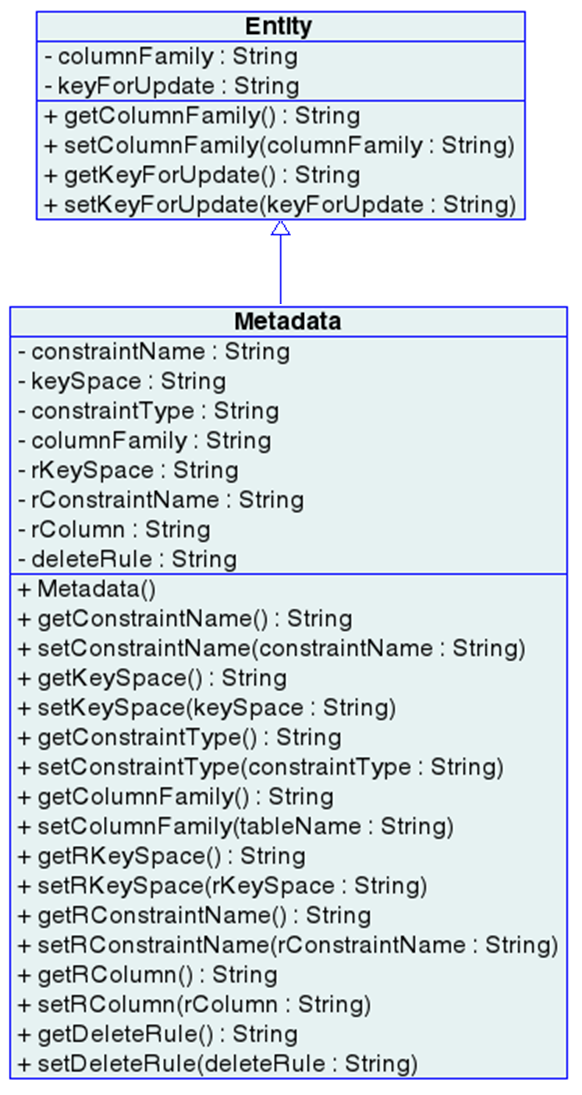
\includegraphics[width=0.6\textwidth]{./figure/Solutions/FinalMetadata.png}
		\caption{Metadata Entity Class}\label{fi:MetadataEntityClass}
	\end{figure}


In order to validate referential integrity in the solutions,  the values of the
constraints applied on an entity have to be retrieved and accessed from
\texttt{Metadata} by the handlers in the experimental \ac{API}.  The solutions
that adopt this approach and treat \texttt{Metadata} entity class as a separate
column family to store the constraints are Solutions~3 and 4. 
Solutions~1 and 2 adopt this approach too,  but only as an internal mechanism to
store the values of the constraints of an entity and is explained in the
following section. 

In Solutions~3 and 4,   all the constraints within a keyspace are treated as
entities and inserted into  \texttt{Metadata}.  The constraints are inserted into
\texttt{Metadata}  the same way as entities are inserted into their respective
entity classes,  using the \texttt{insert} operation,  which is designed to
prevent referential integrity validations for metadata entities.  Note that the
users of the experimental \ac{API} provide all the constraints that have to be
inserted into \texttt{Metadata}. 

In order to perform validations in Solutions~3 and 4,  it is essential that the
\texttt{ValidationHandler}  accesses only the relevant constraints of an entity
from all the constraints stored in the \texttt{Metadata} entity class.  To
distinguish the relevant constraints of an entity,  the
\texttt{ValidationHandler} iterates through the constraints of \texttt{Metadata}
and identifies the constraint that have the entity as the value for its
\texttt{ColumnFamily}. 
Consider Figure~\ref{fd:Metadata-Solution3} which shows a few constraints in
\texttt{Metadata}.  In order to locate the constraints of \texttt{Student} entity
class,  the constraints where \texttt{ColumnFamily} contains 
\texttt{Student} have to be identified,  which in this example is constraint \texttt{CONST100}. 

% Thus,  the relevant \ac{PK} and \ac{FK} constraints of an entity are identified
% by the \texttt{ValidationHandler}. 

Once the relevant constraints are
accessed,   the\texttt{ValidationHandler} performs the necessary validations by
accessing the values from the relevant constraints using \texttt{Metadata}
getter methods.  

By design,  Solution~3 saves \texttt{Metadata} within the same cluster while
Solution~4 saves and maintains it in a separate cluster.  Thus,  the
implementation of this approach in Solution~4 requires a few additional
operations.  

Figure~\ref{fd:MetadataCluster-Solution4} illustrates the separate clusters used
in Solution~4,  where to insert constraints into \texttt{Metadata},  a separate
connection is established to the \texttt{MetadataCluster} and to insert the
other entities into their respective entity classes in the keyspace a separate
connection is maintained to the \texttt{KeyspaceCluster}.  Thus,  in Solution~4, 
retrieving the constraints from \texttt{Metadata} requires using the Hector
connection object established for connecting to the~\texttt{MetadataCluster}. 
Additionally,  in Solution~4 the relevant constraints are stored as a list and
maintained as cache till the operation is completed. 
Hence,  all the relevant \ac{PK} and \ac{FK} constraints for an entity class are
stored in the cache and reused for future operations on the entities of that
type. 

Although Solution~4 requires a separate connection and caches the metadata of
an entity,  it uses the same approach as Solution~3 and 
uses \texttt{Metadata} to access the different parts of a constraint using the
necessary setter and getter access methods. 



\subsection{Metadata as Text}\label{ss:implementation-MDText}

This approach is designed to extract and process embedded metadata that is
stored as a part of an entity and hence this approach is adopted by Solutions~1
and 2  to extract the constraint values of an entity.  

In both Solution~1 and 2,  the relevant constraints of an entity are stored as
values of the \texttt{Metadata} column and contain special characters to
identify its various parts. 
% Every time an operation is invoked on an entity its metadata is accessed from
% its \texttt{Metadata} column and loaded as text. 
Whenever an operation is invoked on an entity,  its metadata is accessed from
its \texttt{Metadata} column and read as a string by the
\texttt{Entity}.  Since the \texttt{Metadata} column of an
entity holds all of its relevant constraints,  each constraint and its different
parts are extracted from the string prior to the validation. 
 \texttt{Entity} parses the string in order to extract the values of
the constraints,  where all the special characters used within the metadata are
the delimiters for the string parsing.  Following are the delimiters used for
parsing. 
		\begin{itemize}
		  \item Special characters '\texttt{\{}',  '\texttt{\}}' and '\texttt{;}' are
		  the delimiters for extracting each constraint from the metadata. 
		  \item Special character '\texttt{;}' is the delimiter for identifying each
		  part within a constraint. 
		  \item Special character '\texttt{:}' is the delimiter for extracting the
		  field name and the value of each part of the constraint. 
		\end{itemize}


Thus,  using this  approach,   \texttt{Entity} in Solution~1 and 2   extract the
embedded metadata and the values within a constraint for an entity. 
These solutions then use the approach of saving metadata in \texttt{Metadata}
entity class,  so that metadata can be accessed during validation. 
After parsing metadata in order to extract the values of a constraint,  the
tokenized values are set as the attributes of \texttt{Metadata} using the
respective setter methods.  These values are accessed by the
\texttt{ValidationHandler}using the getter methods of
the \texttt{Metadata} entity class,  whenever an operation on an entity triggers
a referential integrity validation.  

% In order to perform  validations,  the \texttt{ValidationHandler} accesses
% the relevant values of the constraints of an entity, .  
% For instance,  to get the \texttt{DeleteRule} of a constraint applied on an
% entity,  \texttt{ValidationHandler} uses the \texttt{getDeleteRule()} method of
% the \texttt{Metadata} entity class and similarly other  getter methods are used
% to access the various parts of the constraint. 

In Solution 1,   metadata is saved as a part of the entity in the
\texttt{Metadata} column while Solution~2 saves metadata as a top row with the
unique \texttt{RowId} '\texttt{-1}',  which has only the \texttt{Metadata}
column containing the relevant constraints. 
Thus Solution~2 performs an additional operation to retrieve metadata,  by
searching  for the \texttt{RowId} '\texttt{-1}' in the column family.  
